\paragraph{Предел переменной величины.}\label{1938/231} 
%???зачем это
Если дана последовательность 
\[a_1, a_2, a_3,\dots,a_n,\dots,\]
то $n$-й член её $a_n$ можно назвать переменной величиной, значение которой зависит от её номера $n$.
Этим выражением «переменная величина» часто пользуются для упрощения речи.
Так, вместо выражения «дана бесконечная числовая последовательность $a_1, a_2, a_3,\dots,a_n,\dots$», принято говорить «дана переменная величина $a_n$, принимающая последовательно ряд значений $a_1, a_2, a_3,\dots$».
Если пользоваться этим способом выражения, то можно говорить не о пределе последовательности, а о пределе переменной величины.
%Например, если дана последовательность многоугольников, то можно сказать, что «периметр многоугольников стремится к $p$» вместо того, что «последовательность периметров для данной последовательности многоугольников стремится к $p$».???


В таком случае, предложение, доказанное в §~\ref{1938/228}, можно высказать в форме:
«Всякая переменная величина может стремиться лишь к одному пределу».
Это предложение часто высказывают так:
«если даны две переменные величины $a_n$ и $b_n$, причём все значения первой равны соответствующим значениям второй:
$a_1=b_1$,
$a_2=b_2,\dots, a_n=b_n,\dots$, то предел первой величины, конечно, если он существует, равен пределу второй», или короче:
«если две переменные величины равны, то равны и их пределы». %???фраза-путалка???

Предложение (§~\ref{1938/229}) о пределе возрастающей числовой последовательности можно высказать так:
если переменная величина $a_n$ возрастает с возрастанием номера $n$ и в то же время остаётся меньше некоторого постоянного числа, то эта переменная величина имеет предел.






\InsertBoxR{2}{\parbox{3cm}{\centering
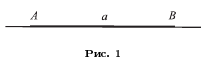
\includegraphics{mppics/ris-1}
\captionof{figure}{}\label{1938/ris-1}
\medskip}}[1]













Изменение размеров фигуры без изменения её формы называется подобным преобразованием данной фигуры.


Построение многоугольника, подобного данному, при заданном коэффициенте подобия называется подобным преобразованием данного многоугольника. %??? не вполне чётко — подобние с поворотом это не подобие??? 














\begin{wrapfigure}{r}{46mm}
\vskip-4mm
\centering
\begin{lpic}[t(0mm),b(0mm),r(0mm),l(0mm)]{jpg/291px-Storchenschnabel_Lokilech(.5)}
\lbl[r]{11,6;$A$}
\lbl[l]{66,6;{$B$}}
\lbl[l]{45,118;$o$}
\lbl[r]{28,152;$a$}
\lbl[l]{48,152;$b$}
\end{lpic}
\caption{}\label{1938/ris-176}
\end{wrapfigure}













\paragraph{Сходственные стороны.}\label{1938/157} %???соответственные???
В этой главе рассматриваются такие треугольники, у которых углы одного соответственно равны углам другого.
Условимся в таких случаях называть сходственными те стороны этих треугольников, которые лежат между соответственно равными углами (такие стороны также и противолежат равным углам).













Значит 
\[\frac{AD'}{D'C}=\frac{AD}{DC}.\]
Следовательно
\[\frac{AD'}{AC}=\frac{AD'}{AD'+D'C}=\frac{AD}{AD+DC}=\frac{AD}{AC},\]
отсюда $AD'=AD$ и значит $D=D'$.
То есть отрезок $BD'$ сливается с биссектрисой угла $B$.

Случай, когда $D'$ лежит на продолжении $AB$ доказывается аналогично.
Не умоляя общности предположить что $AB>BC$, а значит $D'$ лежит на продолжении $AC$ за $C$.
Если $D$ есть точка пересечения биссектрисы внешнего угла то по доказанному (§~\ref{1938/187})
\[\frac{AD'}{D'B}=\frac{AD}{DB}.\]
Следовательно
\[\frac{AD'}{AC}=\frac{AD'}{AD'-D'C}=\frac{AD}{AD-DC}=\frac{AD}{AC},\]
отсюда $AD'=AD$ и значит $D=D'$.
То есть отрезок $BD'$ сливается с биссектрисой внешнего угла $B$.



















\begin{wrapfigure}{r}{35mm}
\centering
\includegraphics{mppics/ris-221}
\caption{}\label{1938/ris-221}
\end{wrapfigure}

\paragraph{}\label{1938/214} %%%???лишнее замечание и картинка не соглсуется с предыдущей???
\mbox{\so{Замечание}.}
Если из центра $O$ (рис.~\ref{1938/ris-221}) опустим на хорды $AB, BC$ и~т.~д.
перпендикуляры и продолжим их до пересечения с окружностью в точках $M, N$ и~т.~д., то эти точки разделяют все дуги и хорды пополам и тем самым разделят окружность на равные части.
Поэтому, если через точки $M, N$ и~т.~д.
проведём касательные до взаимного пересечения, как указано выше, то получим также правильный описанный многоугольник, стороны которого будут параллельны сторонам вписанного многоугольника.
Каждая пара вершин $A$ и $A_1$, $B$ и $B_1$ и~т.~д.
лежит на одной прямой с центром, а именно:
на биссектрисе угла $MON$ и других таких же углов.














\paragraph{Пантограф.}\label{1938/180} %%%???устаревшая секция
Подобное преобразование фигур можно выполнять механически с помощью особого прибора, изобретённого в 1603 году Христофором Шейнером и названного им пантографом. 

\begin{figure}[h]
\centering
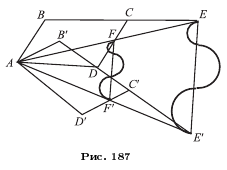
\includegraphics{mppics/ris-187}
\caption{}\label{1938/ris-187}
\end{figure}

Вообразим параллелограмм $ABCD$ (рис.~\ref{1938/ris-187}), сторонами которого служат металлические стержни, могущие на шарнирах вращаться вокруг вершин.
Укрепим неподвижно вершину $A$, возьмём на продолжении $BC$ произвольную точку $E$ и заставим эту точку описать какую-либо линию $EE'$.
Пусть $F$ — точка пересечения прямых $AE$ и $CD$ и $AB'C'D'$ — новое положение нашего шарнирного параллелограмма.
Так как длина сторон параллелограмма и длина отрезков $CE$ и $CF$ при перемещении точки $E$ не изменялись, то можем написать последовательно следующие пропорции:
\[\frac{AD}{CE}=\frac{DF}{FC}=\frac{AF}{FE},\]
так как $\triangle ADF\sim\triangle ECF$,
значит
\[\frac{AD'}{C'E'}=\frac{D'F'}{F'C'}.\]
Отсюда следует, что $\triangle AD'F'\sim\triangle  E'C'F'$;
следовательно, $\angle AF'D'=\angle E'F'C'$, то есть
\so{точки $A$, $F'$ и $E'$ лежат на одной прямой}.
Далее, из подобия тех  же треугольников имеем, что 
\[\frac{AF'}{F'E'}=\frac{D'F'}{F'C'},\]
но
\[\frac{D'F'}{F'C'}=\frac{DF}{FC}=\frac{AF}{FE};\]
следовательно, 
\[\frac{AF'}{F'E'}=\frac{AF}{FE}.\]

Отсюда следует, что треугольники $AEE'$ и $AFF'$ подобны, следовательно, $\angle AFF'=\angle AEE'$ и $EE'\parallel FF'$.


Далее из рисунка находим:
\[\frac{AF}{FE}=\frac{BC}{CE}
\quad\text{и}\quad
\frac{AF'}{F'E'}=\frac{B'C'}{C'E'}.\]

Составляя производные пропорции, можем написать:
\[\frac{AF+FE}{AF}=\frac{BC+CE}{BC}\]
и
\[\frac{AF'+F'E'}{AF}=\frac{B'C'+C'E'}{B'C'}\]
или
\[\frac{AE}{AF}=\frac{BE}{BC}
\quad\text{и}\quad
\frac{AE'}{AF'}=\frac{B'E'}{B'C'}.\]
Но $BE=B'E'$ и $BC=B'C'$, следовательно:
\[\frac{AE}{AF}=\frac{AE'}{AF'}=\frac{BE}{BC}.\]
Это равенство показывает, что когда точка $E$ опишет какую-либо фигуру, точка $F$ опишет подобную фигуру, причём коэффициент подобия этих фигур равен отношению $\frac{BE}{BC}$.
Если в точке $E$ укрепить остриё иглы, а в $F$ — остриё карандаша, то при обводе остриём иглы контура фигуры остриё карандаша зарисует на бумаге контур фигуры подобной.
Для изменения показателя подобия следует переместить точку $E$ по прямой $BC$ в ту или другую сторону.
На этом свойстве шарнирного параллелограмма и основано устройство пантографа, общий вид которого представлен на рис.~\ref{1938/ris-188}.
Прибор применяется при перерисовке планов в различных масштабах.

\begin{figure}[h]
\centering
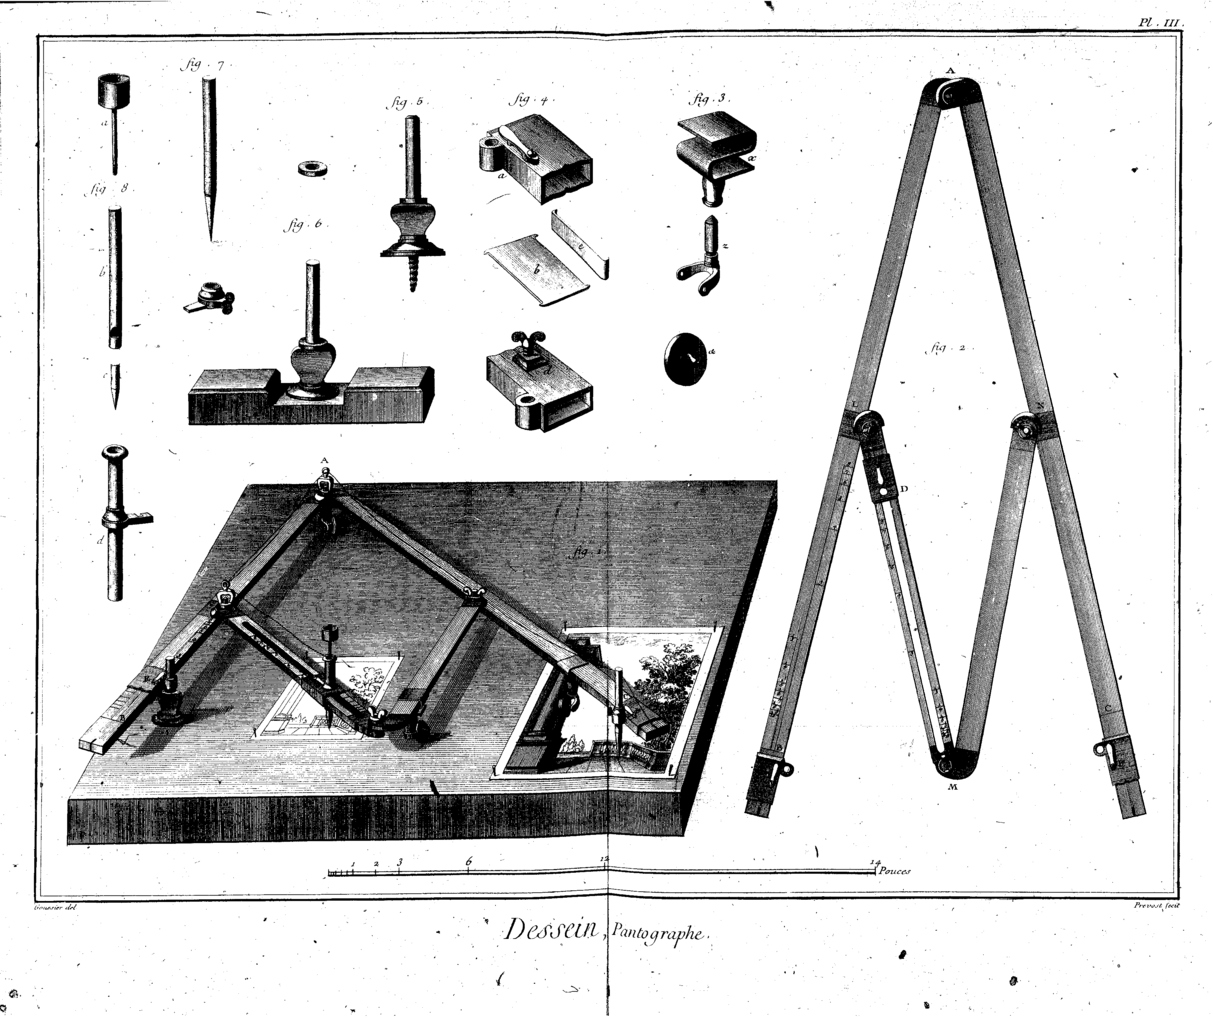
\includegraphics[scale=.25]{jpg/1213px-Encyclopedie_volume_2b-215}
\caption{}\label{1938/ris-188}
\end{figure}

Для подобного преобразования фигур небольшого размера и несложной формы можно пользоваться также делительным циркулем (§~\ref{1938/166}).
Для этого следует установить подвижной винт циркуля так, чтобы он делил всю длину ножки в отношении, равном заданному коэффициенту подобия, затем выбрать центр подобия и соединить его лучами с основными точками фигуры.
На каждом луче следует измерить одним раствором циркуля отрезок от центра подобия до точки фигуры и, перевернув циркуль, отложить на том же луче от центра подобия отрезок, полученный в другом растворе.
Таким способом можно перечертить все основные точки данной фигуры и получить её очертание в нужном размере.





















%вроде лишний пункт???

\paragraph{Сопряжение дуги с прямой или с другой дугой.}\label{1938/116}
При вычерчивании прямых линий и дуг окружностей принято говорить, что отрезок $AB$ (рис.~\ref{1938/ris-129}) и дуга окружности $BC$, сходящиеся в точке $B$, \index{сопряжённые дуги}\textbf{сопряжены}, если в этой точке они касаются и продолжают друг друга.

Две дуги $AB$ и $BC$ (рис.~\ref{1938/ris-130}), сходящиеся в точке $B$, сопряжены, если в этой точке имеют общую касательную $DE$.

\begin{figure}[h!]
\begin{minipage}{.48\textwidth}
\centering
\includegraphics{mppics/ris-129}
\caption{}\label{1938/ris-129}
\end{minipage}
\hfill
\begin{minipage}{.48\textwidth}
\centering
\includegraphics{mppics/ris-130}
\caption{}\label{1938/ris-130}
\end{minipage}
\end{figure}

Для сопряжения прямой с дугой необходимо (§~\ref{1938/113}), чтобы центр окружности, которой принадлежит дуга, лежал на перпендикуляре к прямой, восстановленным из точки сопряжения.

Для сопряжения одной дуги с другой дугой необходимо (§~\ref{1938/113}), чтобы центры двух окружностей, которым принадлежат дуги, лежали на прямой, проходящей через точку сопряжения и перпендикулярной к общей касательной этих дуг.

Сопряжение двух линий (прямой с дугой или двух дуг) делает переход с одной линии на другую плавным, без выступов;
оно практикуется, например, при устройстве закруглений железнодорожных или трамвайных путей.



 \item
Начертить дугу, сопрягающуюся (§~\ref{1938/116}) с данной прямой в данной точке и проходящую через данную точку.

 \item
Соединить две непараллельные прямые сопрягающей (§~\ref{1938/116}) их дугой.
Рассмотреть три случая:

1) когда точки сопряжения и радиус дуги не даны;

2) когда дан только радиус дуги;

3) когда дана одна точка сопряжения, а радиус не дан (примеры такого соединения прямых дугами представляют «закругления» железнодорожного пути).

\begin{figure}[h!]
\centering
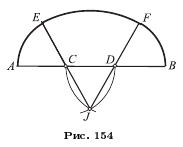
\includegraphics{mppics/ris-154}
\caption{}\label{1938/ris-154}
\end{figure}

\begin{enumerate}[resume]

\item
Линия, называемая в архитектуре «кривой о трёх центрах» (или «полуовальной кривой»), чертится так (рис.~\ref{1938/ris-154}):
делят отрезок $AB$ на три равные части в точках $C$ и $D$;
радиусом, равным $CD$ с центрами в этих точках, высекают дуги в точке $J$;
проводят прямые $JC$ и $JD$ и их продолжают;
описывают дуги $AE$ и $BF$ с центрами в точках $C$ и $D$ и дугу $EF$ с центром в точке $J$.
Объяснить, почему дуги $AE$, $EF$ и $FB$ сопрягаются.
Сопрягались бы они и тогда, когда $AC$ было бы равно $DB$, но не равно $CD$?

 \item
Начертить дугу сопрягающуюся (§~\ref{1938/116}) с данной прямой в данной точке и проходящую через данную точку.















\paragraph{Делительный циркуль.}\label{1938/166} %???можно без этого пункта обойтись???
На подобии треугольников основано употребление делительного циркуля, посредством которого можно быстро разделить данный небольшой отрезок на несколько равных частей.

Прибор этот состоит из двух одинаковых ножек (рис.~\ref{1938/ris-176}) $Ab$ и $Ba$, концы которых заострены.
Вдоль ножек сделаны прорезы, в которых можно передвигать подвижный винт и закреплять его в том или другом месте ножек.
Ножки можно раздвигать и сближать, вращая их вокруг винта.
Положим, требуется разделить отрезок $AB$ на три равные части.
Для этого укрепим винт в такой точке $o$, чтобы расстояние $Ao$ было в 3 раза более расстояния $oB$ (что легко выполнить по тем делениям и цифрам, которые проставлены по краям прореза).
Затем растворяем циркуль и располагаем его так, как указано на рисунке.
Тогда расстояние между остриями $a$ и $b$ будет составлять $\tfrac13$ длины $AB$, так как из подобия треугольников $AoB$ и $aob$ следует:
\[\frac{ab}{AB}=\frac{ob}{oA}=\frac 1 3\]

Остаётся затем, перевернув циркуль, отложить на отрезке $AB$ 3 раза отрезок $ab$.

\paragraph{Поперечный масштаб.}\label{1938/167}
На свойствах подобных треугольников основано также приготовление поперечного масштаба, устройство которого понятно из рис.~\ref{1938/ris-177}.

\begin{figure}[h!]
\centering
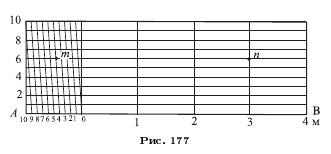
\includegraphics{mppics/ris-177}
\caption{}\label{1938/ris-177}
\end{figure}

Пусть крупные деления линии $AB$ представляют в уменьшенном виде метры.
Тогда мелкие деления представляют дециметры.
Чтобы получить сантиметры, пришлось бы подразделить мелкие деления ещё на 10 равных частей, что, по причине малости этих частей, было бы невыполнимо на линейном масштабе (то есть на самой линии $AB$).
Поперечный масштаб позволяет отсчитывать и сантиметры.

\begin{wrapfigure}[8]{r}{26mm}
\centering
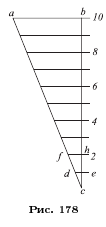
\includegraphics{mppics/ris-178}
\caption{}\label{1938/ris-178}
\end{wrapfigure}

Для разъяснения этого изобразим отдельно в поперечно растянутом виде (рис.~\ref{1938/ris-178})
тот узкий прямоугольный треугольник — самый правый на нашем рисунке. 
Параллельные линии отсекают от этого треугольника подобные треугольники, и потому мы можем написать пропорции:
\begin{align*}
\frac{de}{ab}&=\frac{ce}{cb}=\frac1{10};
\\
\frac{fh}{ab}&=\frac{ch}{cb}=\frac{2}{10}\quad\text{и так далее}
\intertext{значит}
de&=\tfrac1{10}ab;
\\
fh&=\tfrac2{10}ab\quad\text{и так далее}
\end{align*}
Теперь понятно, что если мы возьмём на нашем масштабе циркулем отрезок, положим, от точки $m$ до точки $n$ (рис.~\ref{1938/ris-177}), то этот отрезок составит.
\[3 \text{м}\  4 \text{дм}\  6 \text{см} = 3{,}46\text{м}.\]















 \item
Параллельно прямой, соединяющей центры $O$ и $O'$ двух равных окружностей, проведена секущая, которая с первой окружностью пересекается в точках $A$ и $B$, с второй окружностью — в точках $A'$ и $B'$.

Доказать, что $AA' = BB' = OO'$. %???неоднозначность определения — может случиться что AA'<OO'<BB'???













\begin{wrapfigure}{R}{60mm}
\centering
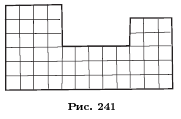
\includegraphics{mppics/ris-241}
\caption{}\label{1938/ris-241}
\end{wrapfigure}

Иногда, поступая описанным способом, мы можем получить точную меру площади.
Это будет, например, тогда, когда контур данного многоугольника представляет собой ломаную линию (рис.~\ref{1938/ris-241}), стороны которой совпадают с частями прямых линий, образующих сеть квадратов; в этом случае, следовательно, не будет совсем квадратов, прорезаемых контуром квадратов, и потому составит точную меру измеряемой площади.

В остальных случаях указанный приём измерения
дает только приближённые результаты.













Тогда, если контур данного многоугольника представляет собой ломаную линию (рис.~\ref{1938/ris-241}), стороны которой совпадают с частями прямых линий, образующих сеть квадратов, то число квадратов, лежащих внутри многоугольника, составит точную меру измеряемой площади.











\section{Тригонометрические функции острого угла}

%??? эта секция была добавлена в поздних изданиях и существенно сокращена в редакции Глагольева; она нигде дальше не изпользуется — разумно дополнить её матерьялом из старой версии и выделить как доп. главу. 

\paragraph{}\label{1938/203}
\so{Определение}.
Пусть $\alpha$ будет какой-нибудь острый угол (рис.~\ref{1938/ris-211}).
Возьмём на одной из его сторон произвольную точку $M$ и опустим из неё перпендикуляр $MN$ на другую сторону угла.
Тогда мы получим прямоугольный треугольник $BMN$.
Возьмём отношения сторон этого треугольника попарно, а именно:
\[\frac{MN}{BM},\]
то есть отношение катета, противолежащего углу $\alpha$, к гипотенузе;
\[\frac{BN}{BM},\]
то есть отношение катета, прилежащего к углу $\alpha$, к гипотенузе;
\[\frac{MN}{BN},\]
то есть отношение катета, противолежащего углу $\alpha$, к катету прилежащему, и им обратные отношения:
\[\frac{BM}{MN}, \frac{BM}{BN}, \frac{BN}{MN}.\]

\begin{wrapfigure}{r}{50mm}
\centering
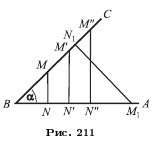
\includegraphics{mppics/ris-211}
\caption{}\label{1938/ris-211}
\end{wrapfigure}

Величина каждого из этих шести отношений не зависит от положения точки $M$ на стороне $BC$.
Действительно, если мы вместо точки $M$ возьмём другие точки $M', M'',\dots$
и опустим перпендикуляры $M'N', M''N'',\dots$, то образовавшиеся треугольники $BM'N'$,  $BM''N'',\dots$
будут подобны треугольнику $BMN$, так как соответственные углы их одинаковы.
Так как в подобных треугольниках сходственные стороны пропорциональны, то 
\begin{align*}
\frac{MN}{BM}&=\frac{M'N'}{BM'}=\frac{M''N''}{BM''}=\dots
\\
\frac{BN}{BM}&=\frac{BN'}{BM'}=\frac{BN''}{BM''}=\dots\quad\text{и так далее}
\end{align*}


Величина каждого из взятых нами отношений не зависит также и от того, на какой стороне угла берётся точка $M$.
Если, например, мы возьмём точку $M_1$ (тот же рисунок) на стороне $BA$ и проведём $M_1N_1\perp BC$, то треугольник $BM_1N_1$ также будет подобен $\triangle BMN$, так как у них имеются по два равных угла, именно по прямому углу и по острому $\alpha$, который входит и в тот, и в другой треугольник;
поэтому
\[\frac{M_1N_1}{BM_1}=\frac{MN}{BM}=\dots\quad\text{и так далее}\]
Таким образом, взятые нами отношения не меняются при изменении положения точки $M$ на этой или другой стороне угла $\alpha$, но конечно, они изменяются при изменении величины самого угла.

При этом каждому размеру угла соответствует вполне определённое значение каждого из этих отношений.

Поэтому мы можем сказать, что каждое отношение есть \textbf{функция} только угла и характеризует собой величину этого угла. %???

Все указанные отношения принято называть \index{тригонометрические функции}\textbf{тригонометрическими функциями угла}.
Чаще других из 6 отношений берутся следующие 4, которым дали особые названия и особые обозначения.

отношение катета, противолежащего углу $\alpha$, к гипотенузе называется \index{синус}\textbf{синусом} угла $\alpha$ и обозначается $\sin \alpha$.

отношение катета, прилежащего углу её, к гипотенузе называется \index{косинус}\textbf{косинусом} угла $\alpha$ и обозначается $\cos\alpha$.

отношение катета, противолежашего углу $\alpha$ к катету, прилежащему к нему, называется \index{тангенс}\textbf{тангенсом} угла $\alpha$ и обозначается $\tg\alpha$.

отношение прилежащего катета к противолежащему (то есть отношение, обратное тому, которое называется тангенсом) называется \index{котангенс}\textbf{котангенсом} угла $\alpha$ и обозначается $\ctg\alpha$.

Так как каждый из двух катетов меньше гипотенузы, то синус и косинус всякого угла есть число, меньшее единицы, и так как один катет может быть и больше, и меньше другого катета, и равен ему, то тангенс и котангенс могут выражаться числами и б\'{о}льшими 1, и меньшими 1, и равными 1. 

\paragraph{Построение угла по заданной величине одной из его тригонометрических функций.}\label{1938/204}\ 

\begin{wrapfigure}{r}{50mm}
\centering
\includegraphics{mppics/ris-212}
\caption{}\label{1938/ris-212}
\end{wrapfigure}

1) Пусть требуется начертить угол, синус которого равняется $\tfrac34$. Для этого надо построить такой прямоугольный треугольник, у которого отношение одного из катетов к гипотенузе равнялось бы $\tfrac34$, и взять в этом треугольнике тот из острых углов, который противолежит этому катету.

{\sloppy

Чтобы построить такой треугольник, возьмём какой-нибудь небольшой отрезок и отложим отрезок $AB$ (рис.~\ref{1938/ris-212}), равный четырём таким отрезкам.
На $AB$ как на диаметре опишем полуокружность.
Далее, радиусом, равным $\tfrac34\cdot AB$ и с центром в точке $B$, опишем дугу до пересечения её в точке $C$ с полуокружностью.
Соединив $C$ с $A$ и с $B$, мы получим прямоугольный треугольник, угол $A$ которого и будет иметь синус $\tfrac34$. %%%можно проще???

}

2) Дано уравнение:
$\cos x = 0{,}7$;
построить угол $x$.
Эта задача решается так же, как и 1-я:
за гипотенузу возьмём отрезок $AB$ (тот же рисунок), равный 10 каким-нибудь одинаковым частям, а за прилежащий катет $AC$ отрезок в 7 таких же частей;
тогда угол $A$, прилежащий к этому катету, и будет искомый.

\begin{wrapfigure}{r}{30mm}
\centering
\includegraphics{mppics/ris-213}
\caption{}\label{1938/ris-213}
\bigskip
\includegraphics{mppics/ris-214}
\caption{}\label{1938/ris-214}
\end{wrapfigure}

3) Построить угол $x$, зная, что $\tg x=1\tfrac12$.
Для этого надо построить такой прямоугольный треугольник, у которого один катет был бы в $1\tfrac12$ раза более другого катета.
Построив прямой угол (рис.~\ref{1938/ris-213}), отложим на одной стороне его произвольной длины отрезок $AB$, а на другой стороне отрезок $AC$, равный $1\tfrac12\cdot AB$.
Соединив точки $B$ и $C$, получим угол $B$, тангенс которого равен $1\tfrac12$.

Такое же построение придётся выполнить, когда угол требуется построить по данному котангенсу, только тогда за искомый угол надо взять тот, который прилежит к катету $AC$.

\paragraph{Изменение тригонометрических функций при изменении угла от 0 до 90\textdegree.}\label{1938/205} %%%??? 205 и 206 выподают из общего строгого стиля книжки
Чтобы удобнее проследить изменение синуса и косинуса при изменении величины угла, мы предположим, что при этом изменении длина гипотенузы остаётся постоянной, равной единице длины, а изменяются только катеты.
Опишем радиусом $AO$ (рис.~\ref{1938/ris-214}), равным произвольной единице длины, четверть окружности $AM$ и в ней возьмём какой-нибудь центральный угол $AOB=\alpha$.
Опустив из $B$ на радиус $OA$ перпендикуляр $BC$, мы будем иметь:
\begin{align*}
\sin\alpha&=\frac{BC}{OB}=\frac{BC}{1}=\text{числ. велич.}\ BC;
\\
\cos\alpha&=\frac{OC}{OB}=\frac{OC}{1}=\text{числ. велич.}\ OC.
\end{align*}
Вообразим теперь, что радиус $OB$ вращается вокруг центра $O$ в сторону, указанную на рисунке стрелкой, начиная от $OA$ и кончая $OM$.
Тогда угол $\alpha$ будет увеличиваться от 0 до $90\degree$ (переходя через указанные на рисунке значения $AOB$, $AOB'$, $AOB''$ и~т.~д.);
численная величина катета $OC$, противолежащего углу $\alpha$, будет увеличиваться от 0 (при $\alpha=0\degree$) до 1 (при $\alpha=90\degree$);
численная величина катета $OC$, прилежащего к углу $\alpha$, будет, наоборот, уменьшаться от 1 (при $\alpha=0\degree$) до 0 (при $\alpha=90\degree$).
Таким образом, \textbf{при возрастании угла от 0 до {90\textdegree} синус его увеличивается от 0 до 1, а косинус уменьшается от 1 до 0.}

\begin{wrapfigure}{R}{30mm}
\centering
\includegraphics{mppics/ris-215}
\caption{}\label{1938/ris-215}
\end{wrapfigure}

Проследим теперь изменение тангенса.
Так как тангенс есть отношение катета, противолежащего углу, к катету прилежащему, то удобнее будет предположить, что при изменении острого угла прилежащий катет остаётся неизменным, равным единице длины, а другой катет изменяется.
Возьмём отрезок $OA$, равный единице длины (рис.~\ref{1938/ris-215}), и примем его за неизменный катет треугольника $AOB$, острый угол которого $AOB=\alpha$ станем изменять.

Согласно определению, 
\[\tg\alpha = \frac{AB}{OA} =\frac{AB}{1} = \text{числ. велич.}\ AB.\]

Будем теперь перемещать точку $B$ вдоль $AN$, начиная от $A$, всё выше и выше через положения $B', B'',\dots$ и~т.~д.;
тогда, как видно из рисунка, угол $\alpha$ и его тангенс будут возрастать, причём когда подвижная точка $B$ совпадает с $A$, угол $\alpha$ равен $0\degree$ и тангенс его будет также 0.
Когда точка $B$ поднимается по прямой $AN$ всё выше и выше, угол $\alpha$ возрастает, стремясь к углу $AOM=90\degree$, и численная величина тангенса тоже возрастает, причём она, очевидно, может сделаться больше какого угодно большого числа (возрастает неограниченно). %???используется темин «стремиться» ДО введения пределов
Значит, \textbf{при возрастании угла от 0 до 90\textdegree{} тангенс его увеличивается от 0 неограниченно.}

Заметим, что вместо того, чтобы говорить о какой-нибудь изменяющейся величине, что она возрастает неограниченно, говорят иначе, что она возрастает до бесконечности, причём слово «бесконечность» выражают письменно знаком $\infty$;
так что изменение тангенса можно выразить так:
при возрастании угла от 0 до $90\degree$ тангенс его возрастает от 0 до $\infty$.

Из определения котангенса (§~\ref{1938/203}) следует, что котангенс есть величина, обратная тангенсу ($\ctg\alpha = \tfrac1{\tg\alpha}$), а потому, когда $\tg\alpha$ возрастает от 0 до $\infty$, то $\ctg\alpha$ убывает от $\infty$ до 0.

\paragraph{Таблица тригонометрических функций.}\label{1938/206} %??? наверно не нужная секция, как и таблицз???
В конце этой книги (страница \pageref{trig-tablitza})
приложена таблица, в которой вписаны тригонометрические функции (с точностью до 5-го десятичного знака) для всех углов, выражаемых целым числом градусов, от 1 до $90\degree$.
Таблица эта расположена так:
в первой слева колонне (над которой напечатано «градусы») помещены числа градусов:
$1\degree, 2\degree, 3\degree,\dots$ до $45\degree$;
во второй колонне (над которой напечатано «синусы») выставлены величины синусов, соответствующие углам, указанным в первой колонне;
в 3-й колонне помещены величины косинусов, затем тангенсов и далее котангенсов, в последней, 6-й колонне помещены снова числа градусов, именно:
$90\degree, 89\degree , 88\degree , 87\degree$ и~т.~д.
до $45\degree$.
Сделано это (ради экономии места) на том основании, что, как следует из определения синуса и косинуса §~\ref{1938/203}, $\sin\alpha=\cos(90\degree-\alpha)$, $\cos\alpha=\sin(90\degree-\alpha)$ и~т.~д.;
значит, $\sin1\degree = \cos 89\degree$, $\sin 2\degree = \cos 88\degree$ и~т.~д.
Поэтому внизу той колонны, над которой сверху стоит надпись «синусы» напечатано «косинусы»;
внизу той колонны (3-й слева), над которой помечено «косинусы», стоит «синусы» и так далее.
Таким образом, для углов от 1 до $45\degree$ надо читать числа градусов в первой колонне слева, а названия тригонометрических функций — над колоннами, для углов же от 45 до 89\degree надо числа градусов брать в последней колонне справа, а названия функций читать внизу колонны.
Например, из таблицы находим:
$\tg35\degree \approx 0{,}70021$, 
$\cos 53\degree \approx 0{,}60182$, 
$\tg72\degree \approx 3{,}07768$.

При помощи такой таблицы мы можем не только %??? приближённо???
находить тригонометрические функции данного угла, но и, наоборот, по данной функции неизвестного угла можем находить (приближённо) этот угол.
Пусть, например, требуется найти угол $x$, зная, что \[\sin x = 0{,}61523.\]
Ищем в колоннах синусов число, возможно близкое к $0{,}61523$.
Это число — $0{,}61566$, означающее приближённое значение $\sin38\degree$.
Так как $0{,}61523<0{,}61566$, то $x < 38\degree$.
Но, с другой стороны, $0{,}61523>0{,}60182$ (последнее число в таблице стоит над числом $0{,}61566\approx\sin37\degree$);
поэтому $x > 37\degree$.
Мы нашли, таким образом, два угла:
$37\degree$ и $38\degree$, между которыми заключается угол $x$.
Значит, если мы вместо $x$ примем угол в $37\degree$ или угол в $38\degree$, то в первом случае найдём приближённое значение с недостатком, а во втором случае с избытком, в том и другом случае с точностью до~$1\degree$.
Предпочтительно брать тот из этих двух углов, синус которого менее разнится от данного (в нашем примере лучше взять $38\degree$).

Пусть ещё требуется найти угол $x$ по уравнению:
$\ctg x= 0{,}7826$.
В колоннах котангенсов находим:
$0{,}78129 \approx \ctg52\degree$;
$0{,}80978 \z\approx \ctg51\degree$.
Так как $0{,}80978>0{,}7826>0{,}78129$, то $51\degree < x < 52\degree$, причём $x$ ближе к $52\degree$, и потому лучше принять $x \approx 52\degree$ (с точностью до $1\degree$).

\paragraph{Зависимость между сторонами и углами прямоугольного треугольника.}\label{1938/207}

\begin{wrapfigure}{R}{30mm}
\centering
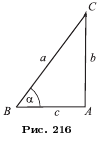
\includegraphics{mppics/ris-216}
\caption{}\label{1938/ris-216}
\end{wrapfigure}

1) Из прямоугольного треугольника $ABC$ находим (рис.~\ref{1938/ris-216}).
\[\frac ba=\sin B,
\quad 
\frac ca=\cos B,
\]
откуда
\[b=a\cdot \sin B,
\quad 
c=a\cdot \cos B.
\]
Так как $B = 90\degree-C$, то 
\[\sin B=\cos C\quad\text{и}\quad \cos B=\sin C;\]
значит, предыдущие равенства можно дополнить так:
\begin{align*}
b&=a\cdot \sin B=a\cdot  \cos C.
\\
c&=a\cdot  \cos B=a\cdot  \sin C.
\end{align*}

Таким образом, \textbf{катет прямоугольного треугольника равен его гипотенузе, умноженной на синус угла, противолежащего этому катету, или на косинус угла, прилежащего к нему.}

2) Из того же треугольника находим:
\[\frac bc=\tg B;
\quad
\frac cb=\ctg B,
\]
откуда
\[b=c\cdot \tg B;
\quad
c=b\cdot \ctg B,
\]
Но 
\[\tg B=\ctg(90\degree-B)=\ctg C
\quad\text{и}\quad
\ctg B=\tg(90\degree-B)=\tg C.
\]
Поэтому можно написать:
\[b=c\cdot \tg B=c\cdot \ctg C;
\quad
c=b\cdot \ctg B=b\cdot \tg C,
\]
то есть \textbf{катет равен другому катету, умноженному на тангенс угла, противолежащего первому катету, или на котангенс угла, прилежащего к нему.}

\paragraph{Решение прямоугольных треугольников.}\label{1938/208}
Указанные зависимости позволяют нам решать прямоугольный треугольник, то есть по некоторым данным элементам его вычислять остальные.
Приведём пример.

\smallskip
\so{Пример}.
В прямоугольном треугольнике известны:
гипотенуза $a = 4{,}5$ и угол $C = 42\degree$.
Найти катеты и угол $B$.
\begin{align*}
b &= a\cdot \cos C = 4{,}5 \cdot \cos 42\degree;
\\
c &= a\cdot \sin C = 4{,}5 \cdot\sin42\degree.\
\end{align*}


Из таблицы находим (ограничиваясь 4 десятичными знаками).
\begin{align*}
\sin42\degree &\approx 0{,}6691,
\\
\cos 42\degree &\approx 0{,}7431.
\end{align*}
Значит:
\begin{align*}
b &\approx 4{,}5\cdot 0{,}7431 = 3{,}34395;
\\
c &\approx 4{,}5\cdot 0{,}6691 = 3{,}01095;
\\
B&=90\degree - C=48\degree.
\end{align*}









При этом могут представиться два различных случая:
или измеряемый отрезок соизмерим с единицей, или несоизмерим с ней.

1) \emph{Измерить отрезок, соизмеримый с единицей, значит узнать, сколько раз в нём содержится единица или какая-нибудь доля единицы.}

\begin{wrapfigure}{R}{48mm}
\centering
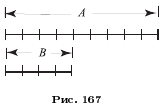
\includegraphics{mppics/ris-167}
\caption{}\label{1938/ris-167}
\end{wrapfigure}







, соизмеримой с $A$.
Тогда находят их общую меру и узнают, сколько раз она содержится в $B$ и $A$.
Если общей мерой окажется сам отрезок $B$, то результат измерения выразится целым числом.
Так, когда $B$ содержится в $A$ три раза, говорят, что длина отрезка $A$ равна 3 единицам.
Если же общей мерой будет некоторая доля $B$, то результат измерения выразится дробным числом.
Так, если общая мера есть $\tfrac14$ доля $B$ и она содержится девять раз (как изображено на рис.~\ref{1938/ris-167}), то говорят, что длина отрезка $A$ равна $\tfrac94$.

Число, получившееся после измерения, называется часто мерой той величины, которая измерялась.
Числа целые и дробные называются \index{рациональное число}\textbf{рациональными числами}.

\begin{figure}[h!]
\centering
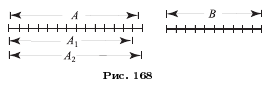
\includegraphics{mppics/ris-168}
\caption{}\label{1938/ris-168}
\end{figure}

2) Когда данный отрезок $A$ несоизмерим с единицей $B$, тогда измерение выполняется косвенно:
вместо отрезка $A$ измеряют два других отрезка, соизмеримых с единицей, из которых один меньше, а другой больше $A$ и которые разнятся от $A$ как угодно мало.
Чтобы найти такие соизмеримые отрезки, 











\medskip

2) Употребим прием доказательства от противного, а именно допустим, что гипотенуза равнобедренного прямоугольного треугольника и его катет его имеют некоторую
наибольшую общую меру $p$, и посмотрим, к чему приведет нас это допущение.

Пусть эта мера $p$ содержится в диагонали $m$ раз и в стороне $n$ раз.
Обратим внимание на то, что целые числа $m$ и $n$ должны быть \so{взаимно простые}, то есть они не должны содержать в себе никакого общего множителя, отличного от $1$
(потому что в противном случае общая мера $p$ не была бы \so{наибольшей}\footnote{Если бы $m$ и $n$ имели бы общий делитель,
например если $m=24$ и $n=15$, то наибольшая общая мера была бы не $p$, а $3p$.}).

По теореме Пифагора, имеем 
\[m^2=2n^2.\]
Значит $m$ должно быть чётным числом; иначе говоря $m=2\ell$ для некого целого $\ell$.
Но тогда 
\[4\ell^2=2n^2\qquad\text{или}\qquad 2\ell^2=n^2,\]
значит $n$ также является чётным.
То есть 2 является общим делителем чисел $m$ и $n$, в частности $m$ и $n$ \so{не взаимно просты}  — противоречие. 
%!!! добавил переписанный вариант из 1931/148 















\paragraph{}\label{1914/228}
\so{Теорема}.
\textbf{\emph{Геометрическое место точек, до которых расстояния от двух данных точек}} ($A$ и $B$ рис. ???) \textbf{\emph{находятся в постоянном отношении $m:n$, есть окружность, когда $m\ne n$, и прямая, когда $m=n$.}}

Предположим сначала, что $m\ne n$.
Тогда на прямой $AB$ (черт. ???), можно найти две точки
принадлежащие искомому геометрическому месту (225???).
Пусть это будут точки $C$ и $C'$ т.~е.
\[\frac{CA}{CB}=\frac{C'A}{C'B}=\frac mn.\]

Предположим теперь, что существует ещё какая-нибудь точка $M$ не лежащая на прямой $AB$ и удовлетворяющая пропорции:
\[\frac{МA}{МB}=\frac mn.\]

Проведя $MC$ и $MC'$ мы должны заключить (???), что первая из этих прямых есть биссектрисса угла $AMB$, а вторая — биссектрисса угла $BMN$;
вследствие этого угол $CMC'$ составленный из двух половин смежных углов, должен быть прямой, а потому вершина его $M$ лежит на окружности, описанной на $CC'$ как на диаметре.

Таким образом, мы доказали, что всякая точка $M$, принадлежащая искомому геометрическому месту, лежит на окружности ???.
Теперь докажем обратное предложение, т.~е., что всякая точка этой окружности принадлежит геометрическому месту.???

Пусть $M$ есть произвольная точка этой окружности.
Требуется доказать, что 
\[\frac{МA}{МB}=\frac mn.\]
Проведя через $B$ прямую $BE\parallel AM$, будем имет следующие пропорции:
\[\frac{MA}{BD}=\frac{C'A}{C'B}=\frac mn \eqno(1)\]
\[\frac{MA}{BE}=\frac{CA}{CB}=\frac mn \eqno(2)\]
Откуда 
\[BD=BE.\]

т.~е. точка $B$ есть середина отрезка $DE$.
Так как угол $CMC'$ вписанный и опирается на диаметр, то он прямой;
поэтому $\triangle DME$ прямоугольный.
Вследствие этого, если середину $B$ гипотенузы $DE$ примем за центр и опишем окружность, то эта окружность пройдет через $M$; значит, $BD=MB$.
Заменив в пропорции (1) на место $BD$ равное  будем иметь:???
\[\frac{МA}{МB}=\frac mn.\]

Когда m = n рассматриваемое геометрическое место, очевидно, обращается в срединный перпендикуляр к отрезку $AB$.

\so{Замечание}.
Окружность, о которой говорится в этой теореме, известна под названием \index{окружность Аполлония}\textbf{окружность Аполлония} (Аполлоний — греческий геометр, живший за 2 вeка до нашей эры).